\documentclass[10pt,a4paper]{report}

\usepackage[latin1]{inputenc}
\usepackage{hyperref}
\usepackage{graphicx}

\hypersetup{colorlinks=true, linkcolor=black, citecolor=black, urlcolor=black}

\author{Hildeberto Mendon\c{c}a}
\title{JUG Management Application}

\begin{document}

\maketitle

\tableofcontents

\part{User Guide}

%\chapter{Introduction}

%\section{The Art of Managing a Java User Group}

%* Can you tell us about the application, site, or service in which you have
%  adopted GlassFish?
%   [ Note: this is where you can hopefully get some publicity for your
%     own business or project.  So consider including any hyperlinks,
%     screenshots, etc. that you would like for us to use in that context. ]

%\section{An Application to Manage JUGs}

%The JUG Management application explicitly aims to increase and strengthen the Java Community by promoting control of JUG operations and managing the knowledge produced by members of the group. We believe that knowledge and opportunities are the main forces of attraction around Java User Groups and an application is needed to make these forces efficiently flow through the community. It is also important to emphasize that JUG leaders have always been great entrepreneurs, but they lack of analytical information to make mature decisions.

%The CEJUG Community (http://www.cejug.org) is leading the project and decided to make it widely available as an open source software. It is freely available for use and open for contributions. CEJUG is using the first release of the application (http://www.cejug.org:8080/cejug) since January 1st, 2011. It is helping the group to define what is actually being a JUG member. Nowadays, most of JUGs simply consider all those people registered in their technical mailing as members. This simplicity is good for management purposes, but we lose lots of information because of that. We don't know, for instance, which reasons led members to leave the group. Did we do something wrong? What can we do to get better and have members back into the boat? We also noticed that even non-technical people, as entrepreneurs, recruiters, and those who decided to unsubscribe because of too many messages, would like to keep in touch with the group, not necessarily going into technical discussions, but proposing other ways of collaboration. Adopting a separate application to manage subscriptions is helping CEJUG to collect more feedback and be more inclusive.

\chapter{Membership Management}

\section{Registration}

The decision to register in the user group always come from the interested person. That is why the only way to add a new member is filling out the initial registration form, accessible through a link in the application header when there is no member logged in. JUG leaders do not have any feature that allow them to add new members manually.

Besides the basic personal data, the registration form also asks the interested person to select one or more of the following options:
\begin{itemize}
\item ``\textit{I want to be aware of all events organized and supported by the UG in a local, national and international level}'' - as a member, the person will receive information about events organized by the UG (see chapter \ref{chp:event-management}) and other supported events promoted by partners and sponsors.
\item ``\textit{I want to receive sponsors' and supporters' offers of products and services, such as books, courses, magazines, etc}'' - only those members who checked this option will be able to participate in raffles, promotions and other contests promoted by sponsors.
\item ``\textit{I want to receive local and national job offers related to Java}'' - only those members who checked this option will receive job offers from partners and sponsors.
\item ``\textit{I want to participate in the technical discussion list}'' - checking this option, the member will be automatically registered in the technical mailing list.
\item ``\textit{I want to receive news about Java and other related technologies, as well as news about the market and other communities}'' - only those members who checked this option will receive news about subjects discussed in the group and other community activities.
\item ``\textit{Other UG members will be able to see my profile and contact me directly through the application. The application will carefully protect the email address, not showing it for others}'' - only members who checked this option will be able to use the social features of the application.
\end{itemize}

When the interested person submits the registration form, we have to make sure that his/her email address is correct before considering him/her as a member. We send an email message to the email address informed in the form, asking the interested person to confirm their email address by clicking on the confirmation link. This link contains a unique code that guarantees that the link cannot be reused after its first use, confirming the email address only once. The interested person is considered as a member as soon as his/her email address is confirmed. The new member receives a welcome email message and JUG Leaders are informed by email about the successful member registration.

\section{Member Profile}

The member has the right to read and modify any data published on its profile. The email address is the only data subject of validation. The email validation works the same way it works during the registration, sending a message to the new email address with a link to confirm it.

\section{Deactivation}

The deactivation of a member means that he/she will not participate in the activities of the group  starting from the date of the deactivation. No email message, invitation, offer, or any other kind of information will be sent to the deactivated member anymore. Therefore, he/she is not considered as a regular member.

At the same time, all data inputed by the ancient member in the database will not be removed. Comments, email messages, articles and other information will be kept unchanged indefinitely. Therefore, any modification on these data is not responsibility of the application.

\part{Developer Guide}

\chapter{Software Architecture}

JUG Management should be deployed in an Application Server (AS). This platform is responsible for the system execution, the connectivity to several resources available in the environment and the availability for several users and systems. For the moment, Glassfish 3.0.1 is the standard AS for this application. This JEE Server has gained lots of attention for constantly run towards the state-of-the-art of the Java server side technology. It has an aggressive roadmap, being always the first product on the market to fully implement the last version of the JEE specification.

No test was performed in other AS up to now, mainly because when the project started Glassfish was the only AS implementing the JEE 6 specification (JPA2, EJB 3.1, JSF 2.0, etc.). The AS should have access and provide the following resources:

\begin{itemize}
\item Security Realm: is a provider of authentication and authorization data to identify users who want to access the application and verify whether they have rights to access protected resources.  The application's database, besides storing UG's data, also stores users and their roles, which makes it the realm provider, referenced by Glassfish in the realm configuration.
\item Database Server: a database driver allows connections to a relational database and a connection pool manages several simultaneous connections to this database, allowing scalability and performance. MySQL is the database system chosen to organize and protect UG's data.
\item Email Server: A JavaMail service connects to an email server and provide sessions to the application, allowing it to send and receive email messages without any special configuration on the implementation side.
\item File System: the application should be able to save and access files in a specific directory of the file system. Unfortunately, the AS does not manage access to the file system. The application is responsible for managing all uploaded files.
\end{itemize}

The resources provided by the application server help to simplify the overall application architecture. The connectivity with those resources characterizes a n-tier architecture, where each tier is physically separated. The application architecture, in turn, is divided in four layers, as depicted in Figure \ref{fig:jug-management-architecture}. These layers provide a model to create a flexible and reusable implementation. This way, new features can be efficiently accommodated, with a minimal impact on existing code.

\begin{figure}
\center
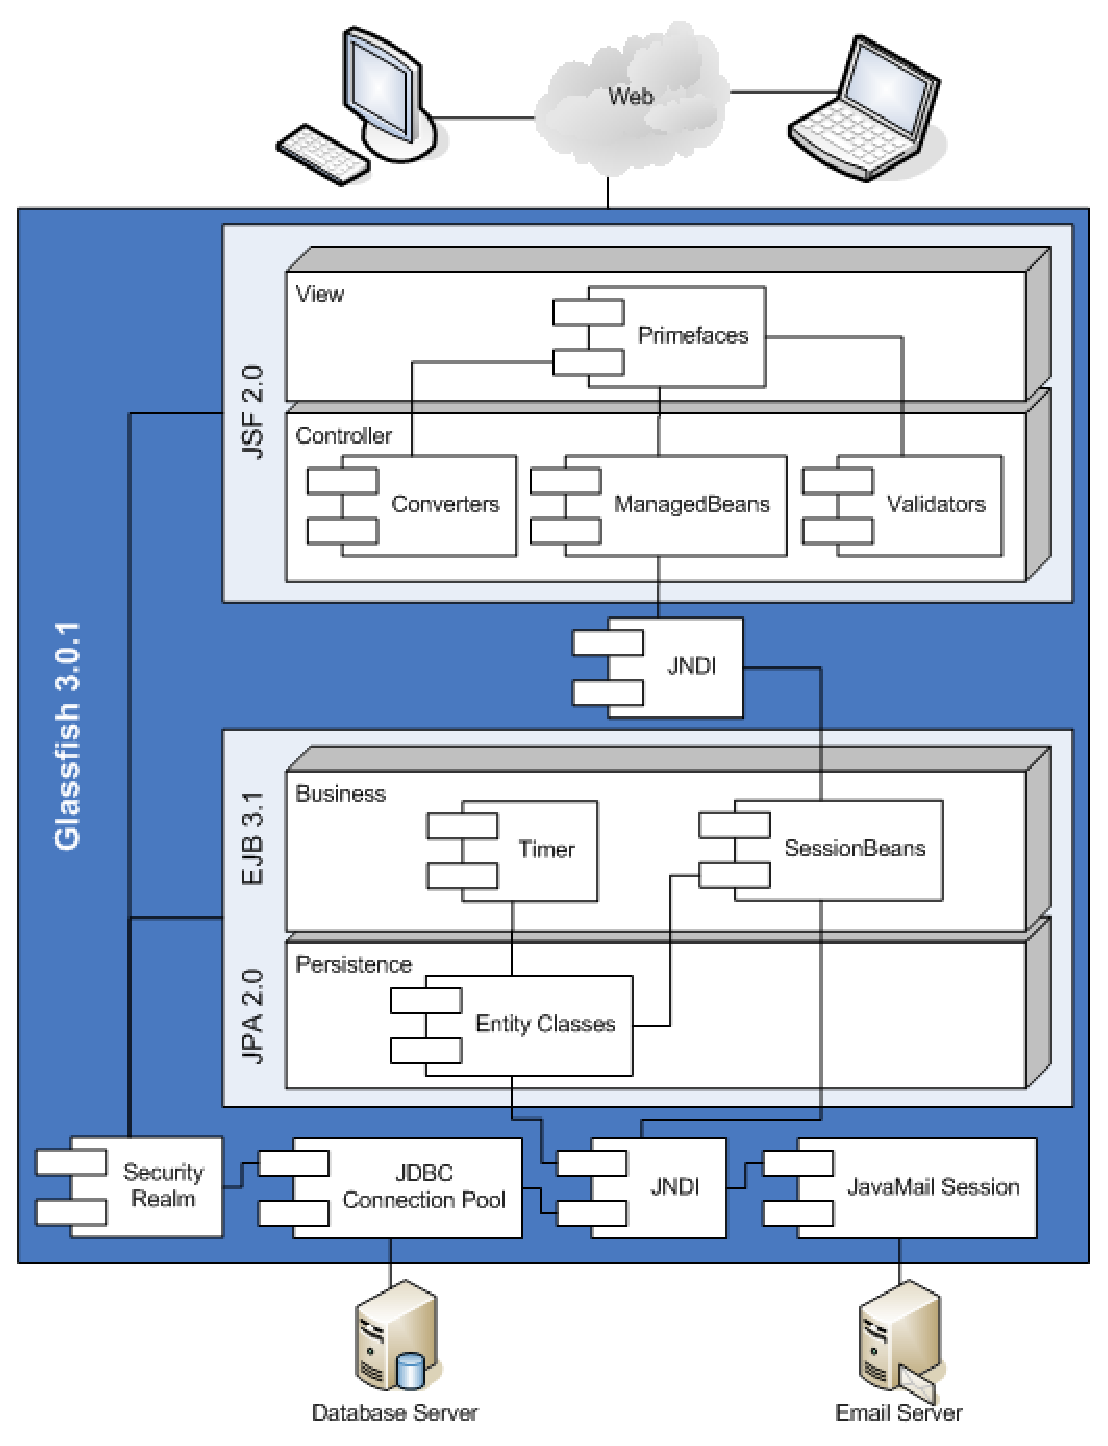
\includegraphics{images/jug_management_architecture}
\caption{JUG Management Architecture}
\label{fig:jug-management-architecture}
\end{figure}

The 4 logical layers are:

\begin{itemize}
\item View: implements the user interface by defining the layout of the screens, position UI components, performing data validation (e.g. invalid date format), formatting data to be presented, internationalizing and localizing text, and giving feedback about the user interaction.
\item Controller: controls the navigation flow according to the user interaction and intermediates data from the view to the business and vice-versa. It performs business validation (e.g. user already exists), data conversion from user friendly to business model-compliant and vice-versa, accesses business services, creates model objects that do not exist yet and manipulates existing ones. According to the state of the IS, the controller knows which flow should be followed and what to do in case of exceptions and security constraints.
\item Business: due to its objectivity, the business layer is not subdivided. It is considered as concrete and it will perform transactional business operations over the data model. Every business operation should guarantee that the data model is consistent before and after its execution. Therefore, the data model can only be access through this layer.
\item Persistence: maps data model entities with database tables to manage the lifecycle of entity objects. These objects can be created (insert), updated (update), queried (select) and deleted (delete). These operations are widely used by the data access object layer in order to interact with the database. The persistence layer can manage one or more data sources, but a data source is managed by one and only one data source.
\end{itemize}

\section{Chosen Technologies}

Table \ref{tbl:chosen-technologies} lists the technologies adopted by the development team to implement the application.

\begin{table}
\begin{center}
\caption{Chosen technologies to implement logical layers}
\label{tbl:chosen-technologies}
\begin{tabular}{p{3cm}p{4cm}p{2cm}}
\hline \noalign{\smallskip}
\textbf{Logical Layer} & \textbf{Technology} & \textbf{Version} \\
\noalign{\smallskip}
\hline
View & JSF Facelets & 2.0 \\
 & Primefaces UI Library & 2.1 \\
Controller & Primefaces & 2.1 \\
 & JSF Managed Bean & 2.0 \\
Business & EJB Session Beans & 3.1 \\
 & EJB Timer & 3.1 \\
Persistence & JPA & 2.0 \\
 & Eclipse Link & 2.0 \\
 & JTA & 1.2 \\
\hline
\end{tabular}
\end{center}
\end{table}

These technologies were selected based on the current needs, resources and knowledge of the development team. We decided to adopt a minimalist approach where most libs needed by the application are also distributed with the AS, such as Eclipse Link and Mojarra, and most configurations are made through the administrative console, such as database connection pool, JavaMail session and Security Realm. For the moment, the only external lib is the Primefaces component library. We make extensive use of annotations and avoid as much as we can XML for configuration purpose. Transactions are fully managed by the container. This way, we keep focused on the source code of the JUG community model. Eventually, other technologies out of this table may be adopted if well justified. Therefore, a new technology would be considered in case a very special UG's need must be fulfilled.

Going into details about the chosen technologies, we describe each one of them, completing the description of Figure \ref{fig:jug-management-architecture}:
\begin{itemize}
\item JSF 2.0: The Java Server Faces technology is the standard technology for developing web-based applications in the JEE platform.
\begin{itemize}
\item Primefaces: extensive library of UI Widgets available for the JSF technology.
\item Converters: converts data from user friendly to business model-compliant and vice-versa.
\item ManagedBeans: POJO annotated classes that have access to special resources available on the application context.
\item Validators: performs server-side validation of data informed by the user before going forward in the controller processing.
\end{itemize}
\item JNDI: the Java Naming and Directory Service helps to localize and retrieve instances of resources available in the context of the server, reusing existing instances and avoiding the complexity behind creating those instances.
\item EJB 3.1: transactional, distributed and secure component model to encapsulate reusable business logic.
\begin{itemize}
\item Stateless Session Beans: EJB that does not store the state of components in memory, optimizing memory allocation and scalability across multiple servers.
\item Timer: EJB capable of scheduling itself to execute business logic in a certain time or in a certain frequency of time. The schedule of routines is very appropriate to perform automatic maintenance tasks such as cleaning temporary data, generating complex reports, sending alert messages, etc. Timers are also useful to efficiently use computational resources when systems are in idle mode.
\item ManagedBeans: POJO annotated classes that have access to special resources available on the enterprise context.
\end{itemize}
\item JPA 2.0: Java Persistence API is an entity-relational mapping specification that manages the lifecycle of objects persisted in the database. It reduces the degree of database dependency, the complexity of the source code and the maintenance cost in case of changes in the relational model.
\end{itemize}

\end{document}